% Guidance - 3 pages
% A technical description of the problem in terms of the requirements given,
% expanded into a discussion and highlighting likely implied technical aspects
% and challenges that need/needed to be tackled


\section{Description of Problem and Requirements}



The Embedded Systems Project consisted of two main sections: a group solution 
that was required to meet a set specification, and an individual extension to 
the group's solution that was left up to each person to determine. 
Both sections of the project involved embedded systems software development in 
the C programming language. 
\par\bigskip\noindent
The target platform of the project is an ARM-based microcontroller, 
situated on a board of peripheral accessories. 
The microcontroller consists of 
an interface board coupled with the ARM cortex-M3 based LPC1768, providing easy 
interaction via USB cable to transfer binaries, and simplifying the process of 
serial communication \cite{how-mbed-works}.
The MBED board is also sat on a board of peripheral accessories, enabling 
interaction with a variety of different components. 
The board is pictured below
\cite{mbed-picture}.
\begin{center}
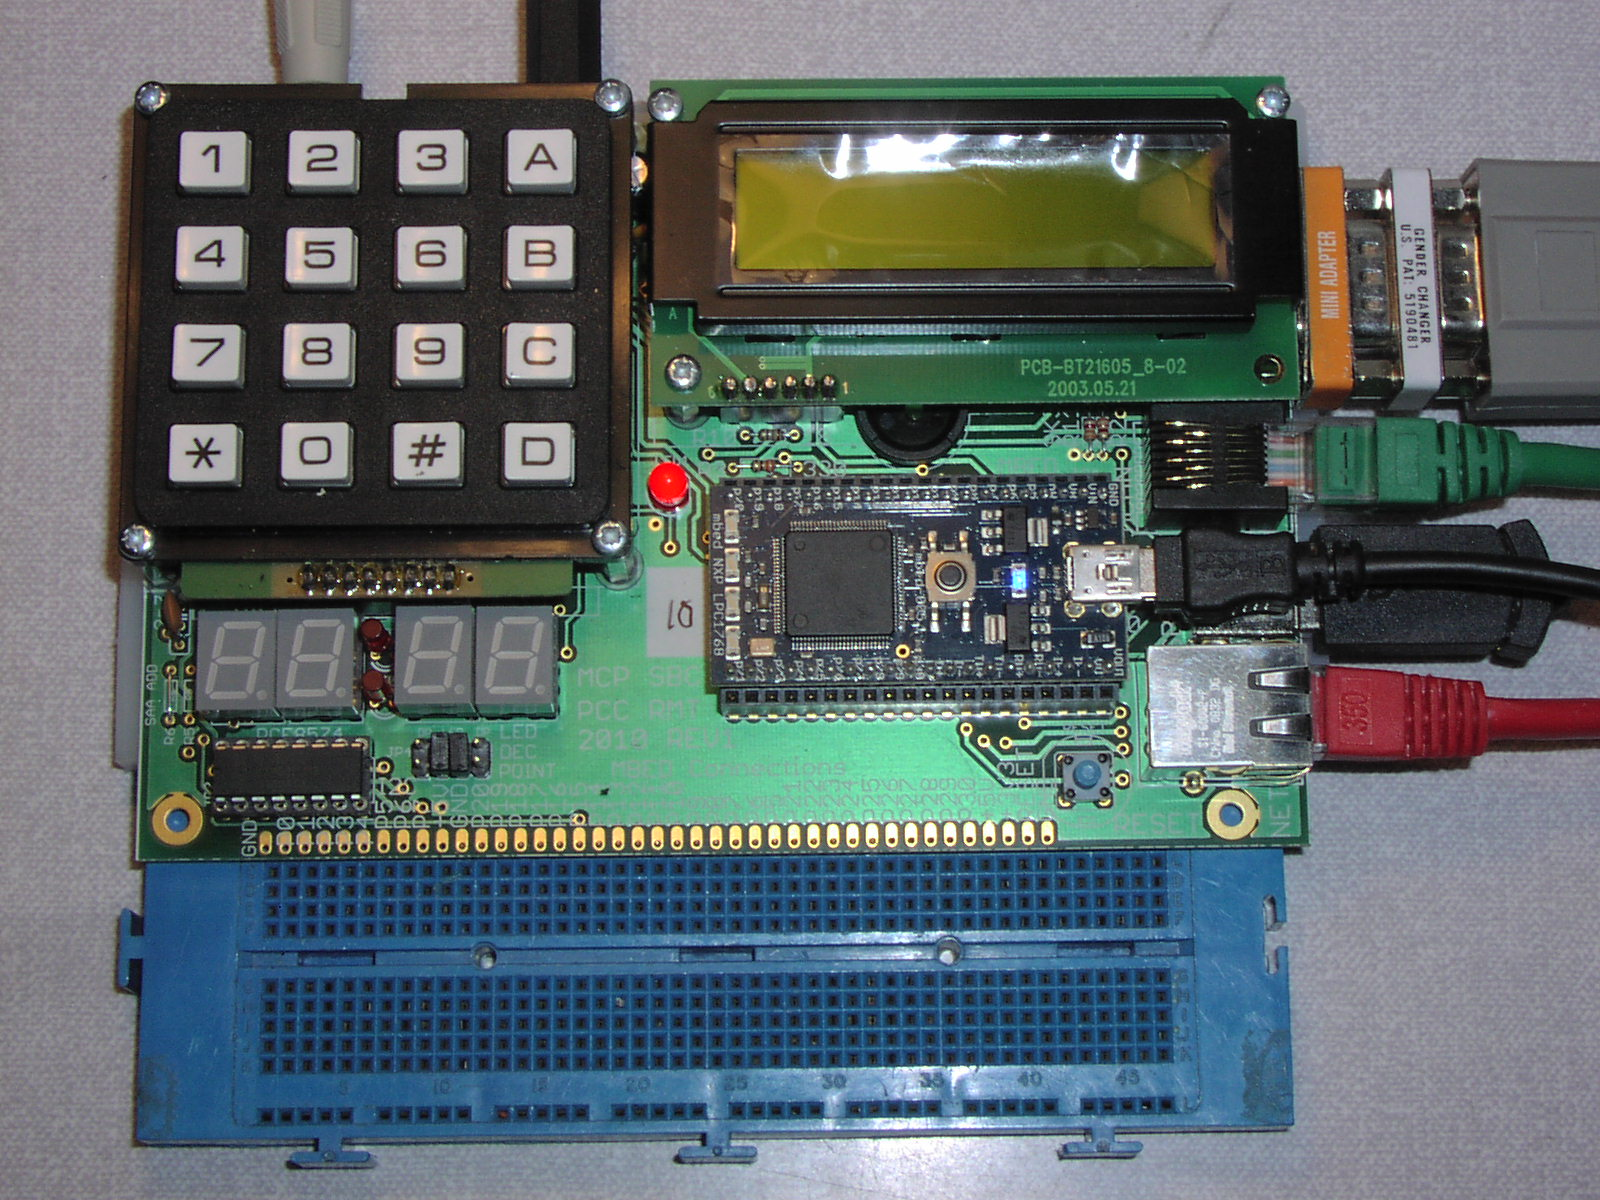
\includegraphics[width=0.80\textwidth]{./mbed_board}
\end{center}
Accessories on the board include: a 16 key keyboard, 
a 16 by 2 line LCD, four seven segment displays, a micro SD slot, a USB host 
connection, CAN bus connector, audio in and out jacks, a TCP/IP connection, as 
well as off board connections to user definable hardware. 
Interaction with these devices is achieved directly through the manipulation of 
the MBED board's pins, therefore enabling a high level of communication with 
relative ease \cite{mbed-pins}. 
The range of devices provides a large variety of possible methods for meeting 
the specification aims, and enables a large scope for individual creativity with 
extensions to the specification.
\par\bigskip\noindent
The group task consisted of multiple different challenges, with the concept
that the MBED board would continually receive data from a controller area network
bus (CAN bus). 
A CAN bus is a type of network, commonly used for rapid 
communication between embedded systems in situations such as aeroplanes and cars.
It could be simply stated as "a network technology that provides fast 
communication among microcontrollers up to real-time requirements" 
\cite{voss2005comprehensible}. 
Following the successful retrieval of CAN packets 
from the network bus, the group solution must decode any packets received, 
filter out those that do not correspond to the selected channel, 
and play notes corresponding to the frequency, volume, and duration specified 
in the received packet.
In addition the user must be able to view useful information, select the channel 
id, and adjust the volume of the device. 
The full requirements for the group solution are as follows 
\cite{specification}:
\par\bigskip\noindent
\textbf{S.1. A solution using MBED for live monitoring of CAN bus data packets.}
\hangindent=0.7cm
Ideally this should include the ability to show all data and also 
to show data filtered according to a configurable instrument channel ID.
\par\bigskip\noindent
\textbf{S.2 An MBED solution which has the following specifications :-}
\begin{itemize}
        \item 
            Receives CAN bus data continuously
        \item 
            Has the ability to preset a local 'ID”
        \item 
            Can optionally filter the data according to it matching the preset ID
        \item 
            For each data element, will generate an audio tone corresponding to frequencies,
            durations, and volume levels if specified in the data stream
        \item 
            Has a visual display on the MBED host board indicating useful information
        \item 
            Has the ability to receive user input via keypad, or an alternative
        \item 
            Has a volume control function
\end{itemize}
\noindent
In addition to the group solution, each individual was required to extend their 
groups implementation.  
This extension did not have to match any set specification, and was instead left 
up to each individual to decide.
For my individual extension, I implemented a shell style user interface. 
This allows user to interact with the device by typing commands into a terminal 
on their computer, effectively adding an additional element of user control that 
is both more intuitive and more responsive than using the 16 digit keypad, from 
the MBED peripherals board.
\par\bigskip\noindent
For our group solution, the specification was broken down into three separate 
areas. 
This allowed us to focus our expertise and interests on the aspect best 
suited to each group member.
The breakdown of the three sections was as follows: 
\begin{itemize}
    \item 
        The receiving and decoding of CAN packets (CAN bus).
    \item 
        Generation of audio samples corresponding to frequency, duration and 
        volume (Audio).
    \item 
        User interaction with the device in order to display information 
        and adjust settings.
\end{itemize}



\section{Discussion of Technical Aspects and Challenges}

My group deconstruced the specification into three major areas requiring 
technical innovation. 
These three main areas, as seen in the previous section, 
equally correspond to the main technical aspects and challenges faced in 
meeting the specification for the group project. 
\par\bigskip\noindent
The first of these challenging areas regarded the receival of data from the CAN 
bus, and the decoding of any packets received to extract their content. 
Data transmitted on the CAN bus does not necessarily arrive at regular intervals, 
and it is impossible to determine when packets may arrive.
Due to the rapid communication the utilisation of the CAN bus enables, it is 
possible for a large number of packets to arrive in a very short space of time.
The ability to receive and process each packet, without any being missed, is 
crucial for the correct functionality of the device. 
This therefore requires a highly optimised, interrupt based solution, capable of
receiving and managing a large amount of data transfer in a very short space of
time. 
Furthermore, the extraction of data from any received packets presents an 
additional technical challenge. 
Received packets may be of a variety of different lengths and types, so a robust 
system must be implemented in order to retreive their data. 
\par\bigskip\noindent
The second technical challenge of the project is the generation of audio tones 
corresponding to frequency, duration and volume levels as specified by the CAN 
packets. 
No information is known about the audio output  apart from the frequency, 
duration and volume of each note. 
The implementation of an audible output therefore requires the generation and 
manipulation of a wave. 
The most logical solution to generating a wave would be the use of a wave lookup 
table, giving values for a range of different values. 
However, this presents additional challenges of storing the wavetable in memory 
on the device, and interpolating between values accurately and rapidly. 
Further areas of technical challenge arise in the production of a more authentic 
sounding product. 
In order to increase the realism of the implemented sound samples, additional 
features such as 'Attack Decay 
Sustain Release' models of a waves lifespan \cite{asr-book}, equal loudness 
curves \cite{kefauver2001audio}, and sound synthesis \cite{miranda2012computer} 
must also be implemented into the solution, vastly increasing the complexity. 
Sound synthesis is a particularly difficult problem, due to the possibility of 
containing expensive mathematical calculations. 
These calculations could slow down the processing of audio samples, resulting in
a strange sounding end product. As a result the efficiency of sound synthesis is 
a vital consideration, and a significant challenge. 
\par\bigskip\noindent
The third technical challenge that can be presented is the ability for a user 
to interact with the device.
The specification determines that the user must be able to control 
the volume of the output, alter which channel of notes is being played, 
and view useful information on the MBED board. 
There are many different methods of interaction with the device, the most 
notable being communication via serial from a desktop computer, or interaction 
through the peripheral accessories provided, such as the 16 digit keypad. 
The user's interaction is not predictable or consistant, and similar to the CAN 
bus data, a large amount of data may be transferred in a short period of time. 
Further challenges are faced as any user interaction with the device requires 
parsing, and executing the required user interaction without having any 
significant effect on the audio output of the system.
Furthermore, the challenge of implementing a user interface is made increasingly 
difficult by the required ability to interact with many other aspects of the 
project. 
Aspects such as the audio synthesis code and the CAN bus code must be carefully 
manipulated and tweaked in order to provide a level of user interaction for 
settings such as the overall output volume, and filtering data from the CAN bus. 
Furthermore any user interface must be both intuitive and user friendly, requiring
careful design considerations. 
